\section{Size Inference}\label{sec:algorithm}

In this section, we present a size inference algorithm, based on that of \CIChat~\citep{cic-hat}.
Starting with a program (that is, a global environment) consisting of bare global declarations,
we want to obtain a program consisting of the corresponding size-annotated global declarations.
Given bare terms corresponding to terms in CIC
(with no size annotations but with the recursive argument index marked on fixpoints),
the algorithm assigns size annotations while collecting a set of subsizing constraints.
Because the subsizing constraints that must be satisfied are based on the typing rules,
this algorithm is also necessarily a type checking algorithm,
ensuring well-typedness of the size-annotated term.
The algorithm then returns either a size-annotated and well-typed term along with the set of subsizing constraints, or fails.

Before proceeding to the next global declaration,
we solve its constraints by finding an assignment from size variables to size expressions
such that these size expressions satisfy all of the constraints.
Then we perform the substitution of these assignments on the declaration.
This lets us run the inference algorithm on each declaration independently,
without needing to manipulate a constraint set every time a global declaration is used in a subsequent one.

One of the most involved parts of the algorithm is the size inference and type checking of \cofixpoints,
which adapts the \RecCheck algorithm from \Fhat~\citep{f-hat}.
The other notably involved part of the algorithm is the \solve algorithm,
which given a set of constraints produces a valid solution.
Finally, we state soundness and completeness theorems for the algorithm as a whole,
proving only soundness and leaving completeness as a conjecture.

\subsection{Preliminaries}

We first formally define the notions of constraints and solutions,
as well as some additional notation.

\begin{definition}
A \textbf{subsizing constraint set} (or simply \textbf{constraint set}) $C$ is a set of pairs of size expressions $s_1 \sqsubseteq s_2$ (also referred to as a \textbf{constraint})
representing a subsizing relation from $s_1$ to $s_2$ that must be enforced.
(When ambiguous, we will explicitly distinguish between the \emph{constraint} $s_1 \sqsubseteq s_2$ and the \emph{judgement} $s_1 \sqsubseteq s_2$.)

We write $s_1 = s_2$ to mean the two pairs $s_1 \sqsubseteq s_2$ and $s_2 \sqsubseteq s_1$.
Given a set of size variables $V$, we also write $\upsilon \sqsubseteq V$ for the pointwise constraint set $\set{\upsilon \sqsubseteq \upsilon' \mid \upsilon' \in V}$,
and similarly for $V \sqsubseteq \upsilon$.
\end{definition}

This is the natural representation of the constraints:
the algorithm is based on the typing rules,
and they produce constraints representing subsizing judgements that need to hold.
However, in \RecCheck and in \solve we will need to view these constraints as a graph.
We use $C$ to represent either the constraint set or the graph depending on the context.
First, notice that any noninfinite size consists of a size variable and some concrete number $n$ of successor ``hats'';
we will write this as $\succ{\upsilon}^n$ so that, for instance, $\succ{\succ{\succ{\upsilon}}}$ is instead $\succ{\upsilon}^3$.

\begin{definition}
A \textbf{subsizing constraint graph} (or simply \textbf{constraint graph}) $C$ of a constraint set is a weighted, directed graph whose vertices are size variables, edges are constraints, and weights are integers.

Given a constraint \mbox{$\succ{\upsilon}_1^{n_1} \sqsubseteq \succ{\upsilon}_2^{n_2}$},
the constraint graph contains an edge from $\upsilon_1$ to $\upsilon_2$ with weight $n_2 - n_1$.
Constraints of the form $s \sqsubseteq \infty$ are trivially true and aren't added to the graph.
Constraints of the form $\infty \sqsubseteq \succ{\upsilon}^n$ correspond to an edge from $\infty$ to $\upsilon$ with weight $0$.
\end{definition}

Given a constraint graph and some set of size variables $V$,
it's useful to know which variables in the graph can be reached from $V$ or will reach $V$.

\begin{definition}[Transitive closures]~\\[-4ex]
\begin{itemize}
  \item Given a set of size variables $V$, the \textbf{upward closure} $\bigsqcup V$ with respect to $C$ is the set of variables that can be reached from $V$ by travelling along the directed edges of $C$.
  That is, $V \subseteq \bigsqcup V$, and if $\upsilon_1 \in \bigsqcup V$ and $\succ{\upsilon}_1^{n_1} \sqsubseteq \succ{\upsilon}_2^{n_2}$, then $\upsilon_2 \in \bigsqcup V$.
  \item Given a set of size variables $V$, the \textbf{downward closure} $\bigsqcap V$ with respect to $C$ is the set of variables that can reach $V$ by travelling along the directed edges of $C$.
  That is, $V \subseteq \bigsqcap V$, and if $\upsilon_2 \in \bigsqcap V$ and $\succ{\upsilon}_1^{n_1} \sqsubseteq \succ{\upsilon}_2^{n_2}$, then $\upsilon_1 \in \bigsqcap V$.
\end{itemize}
\end{definition}

Finally, we can define what it means to be a solution of a constraint set,
as well as some useful related notation.

\begin{definition}[Size substitutions and constraint satisfaction]~\\[-4ex]
\begin{itemize}
  \item A size substitution $\rho$ applied to a set of size variables produces a set of size expressions:
  $\rho V \coloneqq \set{\rho \upsilon \mid \upsilon \in V}$.
  Applying $\rho$ to a constraint set works similarly.

  \item The composition of size substitutions $\rho_1$ and $\rho_2$ is defined as \mbox{$(\rho_1 \circ \rho_2) \upsilon \coloneqq \rho_1(\rho_2 \upsilon)$}.

  \item A size substitution $\rho$ \textbf{satisfies the constraint set} $C$ (or is a \textbf{solution} of $C$), written as $\rho \vDash C$, if for every constraint $s_1 \sqsubseteq s_2$ in $C$, the judgement $\rho s_1 \sqsubseteq \rho s_2$ holds.
  For convenience, we will also require that $\rho$ maps to size expressions whose size variables are fresh,
  and that it does not map any size variables not in $C$.
\end{itemize}
\end{definition}

We now define four judgements to represent \emph{algorithmic subtyping}, \emph{checking}, \emph{inference}, and \emph{well-formed\-ness}.
They all use the symbol $\rightsquigarrow$, with inputs on the left and outputs on the right.
\begin{itemize}
  \item $\gg \vdash t \constrain u \rightsquigarrow C$ (algorithmic subtyping) takes environments $\Gamma_G, \Gamma$ and annotated terms $t, u$, and produces a set of constraints $C$ that must be satisfied in order for $t$ to be a subtype of $u$.
  \item $C, \gg \vdash e^\circ \Leftarrow t \rightsquigarrow C', e$ (checking)
  takes a set of constraints $C$, environments $\Gamma_G, \Gamma$,
  a bare term $e^\circ$, and an annotated type $t$,
  and produces the annotated term $e$ with a set of constraints $C'$
  that ensures that the type of $e$ subtypes $t$.
  \item $C, \gg \vdash e^\circ \rightsquigarrow C', e \Rightarrow t$ (inference)
  takes a set of constraints $C$, environments $\Gamma_G, \Gamma$,
  and a bare term $e^\circ$, and produces the annotated term $e$, its annotated type $t$, and a set of constraints $C$.
  \item $\Gamma_G^\circ \rightsquigarrow \Gamma_G$ (well-formedness) takes a global environment with bare declarations and produces a global environment where each declaration has been properly annotated via size inference.
\end{itemize}

In checking and inference, the input constraint set represents the constraints that must be satisfied
for the local environment to be well-formed.
Algorithmic subtyping does not need this constraint set since subtyping does not rely on well-formedness of the environments.
The output constraint set represents \emph{additional} constraints that must be satisfied
for the input term(s) to be well-typed.

The algorithm is implicitly parameterized over a fixed signature $\Sigma$,
as well as two mutable sets of size variables $\V, \V^*$, such that $\V^* \subseteq \V$.
Their assignment is denoted with $\coloneqq$ and they are initialized as empty.
The set $\V^*$ contains \textit{position} size variables,
which mark size-preserving types by replacing position annotations,
and we use $\tau$ for these position size variables.
We define two related metafunctions: \PV returns all position size variables in a given term,
while $\erase{\ph}^*$ erases position size variables to position annotations and all other annotations to bare.

Finally, on the right-hand size of inference judgements, we use $e \Rightarrow^* t$ to mean $e \Rightarrow t' \wedge t = \whnf{t'}$.
\whnf reduces a term until it is in \emph{weak head normal form} (WHNF),
which allows us to syntactically match on and take apart the term.
A term is in weak head normal form when no reduction rule can be applied to the entire term,
when it has the form $\app{X}{\vec{a}}$ and $X$ is in WHNF,
when it is a case expression whose target is in WHNF,
or when it is an applied fixpoint whose arguments are in WHNF.
For our purposes, the important thing is that we are able to tell whether or not a term is
a universe, a function type, or an inductive type.

We define a number of additional metafunctions to translate the side conditions from the typing rules into procedural form.
They are introduced as needed.

\paragraph*{} The entry point of the algorithm is the well-formedness judgement,
which take and produce global environments representing whole programs.
Its rules are defined in \autoref{fig:algorithm-wf} and use the mutually-defined rules of the checking and inference judgements,
defined in \autoref{fig:algorithm-check}, \autoref{fig:algorithm-core}, and \autoref{fig:algorithm-coind} respectively.
We begin with the latter two first in \autoref{sec:algorithm:infer},
followed by a detailed look at \RecCheck in \autoref{sec:algorithm:reccheck}.
Well-formedness is discussed in \autoref{sec:algorithm:wf}.
Finally, we make our way up to soundness and completeness with respect to the typing rules in \autoref{sec:algorithm:metatheory}.

\subsection{Inference Algorithm}\label{sec:algorithm:infer}

Size inference begins with either a bare term or a position term. For the bare terms, even type annotations of \cofixpoints are bare, \ie
  $$e^\circ \Coloneqq \dots
    \mid \fix{m}{f^n}{t^\circ}{e^\circ}
    \mid \cofix{m}{f}{t^\circ}{e^\circ}$$
Notice that fixpoints still have the indices $n$ of the recursive arguments, whereas surface Coq programs generally have no indices.
To produce these indices, we do what Coq currently does: brute-force search.
We try the algorithm on every combination of indices from left to right.
This continues until one combination works, or fails if none do.
Then the type annotations are initially position-annotated on as many types as possible,
and this position term itself is passed into the algorithm.
Because of the way the Coq kernel is structured, this may not always be possible in the implementation.
We discuss this and other implementational issues in the next section.

\begin{figure*}
\centering
\small

\begin{flushleft}
\fbox{$\cgg \vdash T^\circ \Leftarrow T \rightsquigarrow C, T$}
\end{flushleft}

\vspace{-3ex}

\begin{mathpar}
\inferrule[\defrule{a-check}]{
    \cgp \vdash e^\circ \rightsquigarrow C_1, e \Rightarrow t
}{
    \cgp \vdash e^\circ \Leftarrow u \rightsquigarrow C_1 \cup t \preceq u, e
}
\end{mathpar}
\caption{Size inference algorithm: Checking}
\label{fig:algorithm-check}
\end{figure*}

\begin{figure*}
\centering

\begin{flushleft}
\fbox{$\Gamma_G, \Gamma \vdash t \constrain u \rightsquigarrow C$}
\end{flushleft}

\vspace{-2ex}

\begin{mathpar}
\dots
\and
\inferrule[\defrule{a-st-ind}]
  {I \textrm{ inductive }}
  {\gg \vdash I^s \leq I^{s'} \rightsquigarrow \set{s \sqsubseteq s'}}
\and
\inferrule[\defrule{a-st-coind}]
  {I \textrm{ coinductive }}
  {\gg \vdash I^s \leq I^{s'} \rightsquigarrow \set{s' \sqsubseteq s}}
\end{mathpar}
\caption{Size inference algorithm: Algorithmic subtyping (excerpt)}
\label{fig:algorithm-subtyping}
\end{figure*}

\paragraph*{} \refrule{a-check} in \autoref{fig:algorithm-check} is the checking component of the algorithm.
It uses algorithmic subtyping in \autoref{fig:algorithm-subtyping} to ensure that the inferred type of the term is a subtype of given type.
This subtyping is defined inductively over the rules of the subtyping judgement in the straightforward manner, taking the union of constraint sets from their premises;
we present only Rules \refnorule{a-st-ind} and \refnorule{a-st-coind},
which shows the concrete subsizing constraints derived from comparing two \coinductive types.
It may also fail if two terms are not subtypes and are inconvertible.

\begin{figure*}
\centering

\begin{flushleft}
\fbox{$C, \gg \vdash e^\circ \rightsquigarrow C, e \Rightarrow t$}
\end{flushleft}

\vspace{-4ex}

\begin{mathpar}
\inferrule[\defrule{a-var-assum}]{
    (\assm{x}{t}) \in \Gamma
}{
    C, \gg \vdash x \rightsquigarrow \set{}, x \Rightarrow t
}

\inferrule[\defrule{a-var-def}]{
    (\defn{x}{t}{e}) \in \Gamma \and
    \overline{\upsilon'_i} = \SV(e, t) \setminus \SV(C) \\\\
    \overline{\upsilon_i} = \fresh{\norm{\overline{\upsilon'_i}}} \and
    \rho = \set{\vec{\upsilon'_i \mapsto \upsilon_i}}
}{
    C, \gg \vdash x \rightsquigarrow \set{}, x^\rho \Rightarrow \rho t
}

\inferrule[\defrule{a-const-assum}]{
    (\Assm{x}{t}) \in \Gamma_G
}{
    C, \gg \vdash x \rightsquigarrow \set{}, x \Rightarrow t
}

\inferrule[\defrule{a-const-def}]{
    (\Defn{x}{t}{e}) \in \Gamma_G \and
    \overline{\upsilon'_i} = \SV(e, t) \setminus \SV(C) \\\\
    \overline{\upsilon_i} = \fresh{\norm{\overline{\upsilon'_i}}} \and
    \rho = \set{\vec{\upsilon'_i \mapsto \upsilon_i}}
}{
    C, \gg \vdash x \rightsquigarrow \set{}, x^\rho \Rightarrow \rho t
}

\inferrule[\defrule{a-univ}]{~}{
    C, \gg \vdash U \rightsquigarrow \set{}, U \Rightarrow \axiom{U}
}

\inferrule[\defrule{a-prod}]{
    C, \gg \vdash t^\circ \rightsquigarrow C_1, t \Rightarrow^* U_1 \\\\
    C \cup C_1, \gg (x:t) \vdash u^\circ \rightsquigarrow C_2, u \Rightarrow^* U_2
}{
    C, \gg \vdash \prod{x}{t^\circ\!}{u^\circ} \rightsquigarrow C_1 \cup C_2, \prod{x}{t}{u} \Rightarrow \rules{U_1}{U_2}
}

\inferrule[\defrule{a-abs}]{
    C, \gg \vdash t^\circ \rightsquigarrow C_1, t \Rightarrow^* U \\\\
    C \cup C_1, \gg (x:t) \vdash e^\circ \rightsquigarrow C_2, e \Rightarrow u
}{
    C, \gg \vdash \abs{x}{t^\circ\!}{e^\circ} \rightsquigarrow C_1 \cup C_2, \abs{x}{|t|}{e} \Rightarrow \prod{x}{t}{u}
}

\inferrule[\defrule{a-app}]{
    C, \gg \vdash e_1^\circ \rightsquigarrow C_1, e_1 \Rightarrow^* \prod{x}{t}{u} \\\\
    C, \gg \vdash e_2^\circ \Leftarrow t \rightsquigarrow C_2, e_2
}{
    C, \gg \vdash e_1^\circ ~ e_2^\circ \rightsquigarrow C_1 \cup C_2, e_1 ~ e_2 \Rightarrow u[x \coloneqq e_2]
}

\inferrule[\defrule{a-let-in}]{
    C, \gg \vdash t^\circ \rightsquigarrow C_1, t \Rightarrow^* U \\
    C, \gg \vdash e_1^\circ \Leftarrow t \rightsquigarrow C_2, e_1 \\\\
    C \cup C_1 \cup C_2, \gg (\defn{x}{t}{e_1}) \vdash e_2^\circ \rightsquigarrow C_3, e_2 \Rightarrow u
}{
    C, \gg \vdash \letin{x}{t^\circ}{e_1^\circ}{e_2^\circ} \rightsquigarrow C_1 \cup C_2 \cup C_3, \letin{x}{|t|}{e_1}{e_2} \Rightarrow u[x \coloneqq e_1]
}

\dots

\end{mathpar}
\caption{Size inference algorithm: Inference (1/2)}
\label{fig:algorithm-core}
\end{figure*}

%%% Local Variables:
%%% TeX-master: "../main.tex"
%%% TeX-engine: default
%%% End:


\autoref{fig:algorithm-core} is the first half of the inference component of the algorithm,
presenting the rules for basic language constructs.
In general, when the local environment is extended with some term, we make sure that the input constraint set is extended as well
with the constraints generated from size inference on that term.
The constraints returned are simply the union of all the constraints generated by the premises.
Note that since type annotations need to be bare (to maintain subject reduction, as discussed in \autoref{sec:metatheory:sr:bare}),
they must be erased first before reconstructing the term.

Rules \refnorule{a-var-assum}, \refnorule{a-const-assum}, \refnorule{a-univ}, \refnorule{a-prod}, \refnorule{a-abs}, \refnorule{a-app}, and \refnorule{a-let-in} are all fairly straightforward.
These rules use the metafunctions \axiom, \rules, and \elim, which correspond to the sets \Axioms, \Rules, and \Elims, defined in \autoref{fig:axruel}.
The metafunction \axiom produces the type of a universe; \rules produces the type of a function type given the universes of its argument and return types; and \elim directly checks membership in \Elims and can fail.

In Rules \refnorule{a-var-def} and \refnorule{a-const-def},
we generate a size substitution that freshens the size variables in the associated definition
using $\fresh$, which freshly generates the given number of variables and adds them to $\mathcal{V}$.
By freshening the size variables, we can define let-bound type aliases that can be used like regular types.
For instance, in the term
$$\letin{N}{\Type{}}{\Nat^{\upsilon_1}}{\abs{n}{N \rightarrow N}{n}}$$
the two uses of $N$ need not have the same size:
the type of the function might be inferred as
$N^{\seq{\upsilon_1 \mapsto \upsilon_2}} \rightarrow N^{\seq{\upsilon_1 \mapsto \upsilon_3}}$,
which by $\delta$-reduction is convertible with $\Nat^{\upsilon_2} \rightarrow \Nat^{\upsilon_3}$.

\begin{figure*}[h]
\centering
\small

\begin{flushleft}
\fbox{$C, \gg \vdash e^\circ \rightsquigarrow C, e \Rightarrow t$}
\end{flushleft}

\vspace{-4ex}

\begin{mathpar}
\dots

\inferrule[\defrule{a-ind}]{
    \upsilon = \fresh{1}
}{
    C, \gg \vdash I \rightsquigarrow \set{}, I^\upsilon \Rightarrow \indtype{I}
}

\inferrule[\defrule{a-ind-star}]{
    \tau = \fresh{1} \and \mathcal{V}^* \coloneqq \mathcal{V}^* \cup \set{\tau}
}{
    C, \gg \vdash I^* \rightsquigarrow \set{}, I^\tau \Rightarrow \indtype{I}
}

\inferrule[\defrule{a-constr}]{
    \upsilon = \fresh{1}
}{
    C, \gg \vdash c \rightsquigarrow \set{}, c \Rightarrow \constrtype{c}{\upsilon}
}

\inferrule[\defrule{a-case}]{
    C, \gg \vdash e^\circ \rightsquigarrow C_1, e \Rightarrow^* I_k^s ~ \overline{p} ~ \overline{a} \\
    C, \gg \vdash P^\circ \rightsquigarrow C_2, P \Rightarrow t_p \\
    \prodctx{\any}{\prodctx{\Delta_k}{U_k}} = \indtype{I_k} \\
    U = \decompose{t_p}{\norm{\Delta_k} + 1} \\
    \elim{U_k}{U}{I_k} \\
    \upsilon = \fresh{1} \\
    \gg \vdash t_p \constrain \motivetype{\overline{p}}{U}{I_k^{\hat{\upsilon}}} \rightsquigarrow C_3 \\
    \textrm{For each $j$:} \\
    C, \gg \vdash e^\circ_j \Leftarrow \branchtype{\overline{p}}{c_j}{\upsilon}{P} \rightsquigarrow C_{4j}, e_j \\
    C_5 = \casesize{I_k^s}{\hat{\upsilon}} \cup C_1 \cup C_2 \cup C_3 \cup (\textstyle\bigcup_j C_{4j})
}{
    C, \gg \vdash \caseof{P^\circ}{e^\circ}{c_j}{e_j^\circ} \rightsquigarrow C_5, \caseof{|P|}{e}{c_j}{e_j} \Rightarrow P ~ \overline{a} ~ e
}

\inferrule[\defrule{a-fix}]{
    \textrm{For each $k$:} \\
    C, \gg \vdash t_k^\circ \rightsquigarrow \any, \any \Rightarrow \any \\
    C, \gg \vdash \setrecstars{t_k^\circ}{n_k} \rightsquigarrow C_{1k}, t_k \Rightarrow^* U \\
    \prodctx{\Delta_k}{u_k} = \whnf{t_k} \and \prodctx{\Delta_k}{u'_k} = \shift{\prodctx{\Delta_k}{u_k}} \\
    \textstyle\bigcup_k C_{1k} \cup C, \gg \overline{(f_k : t_k)} \vdash e_k^\circ \Leftarrow \prodctx{\Delta_k}{u'_k} \rightsquigarrow C_{2k}, e_k \\
    \gg \Delta_k \vdash u_k \constrain u'_k \rightsquigarrow C_{3k} \\
    C_4 = \textstyle\bigcup_k C_{1k} \cup C_{2k} \cup C_{3k} \cup C \\
    C_5 = \RecCheckLoop{C_4}{\Gamma}{\overline{\getrecvar{t_k}{n_k}}}{\overline{t_k}}{\overline{e_k}}
}{
    C, \gg \vdash \fix{m}{f_k^{n_k}}{t_k^\circ}{e_k^\circ} \rightsquigarrow C_5, \fix{m}{f_k^{n_k}}{|t_k|^*}{e_k} \Rightarrow t_m
}

\inferrule[\defrule{a-cofix}]{
    \textrm{For each $k$:} \\
    C, \gg \vdash t_k^\circ \rightsquigarrow \any, \any \Rightarrow \any \\
    C, \gg \vdash \setcorecstars{t_k^\circ} \rightsquigarrow C_{1k}, t_k \Rightarrow^* U \\
    \prodctx{\Delta_k}{u_k} = \whnf{t_k} \and \prodctx{\Delta'_k}{u'_k} = \shift{\prodctx{\Delta_k}{u_k}} \\
    \textstyle\bigcup_k C_{1k} \cup C, \gg \overline{(f_k : t_k)} \vdash e_k^\circ \Leftarrow \prodctx{\Delta'_k}{u'_k} \rightsquigarrow C_{2k}, e_k \\
    \gg \vdash \Delta'_k \constrain \Delta_k \rightsquigarrow C_{3k} \\
    C_4 = \textstyle\bigcup_k C_{1k} \cup C_{2k} \cup C_{3k} \cup C \\
    C_5 = \RecCheckLoop{C_4}{\Gamma}{\overline{\getcorecvar{t_k}}}{\overline{t_k}}{\overline{e_k}}
}{
    C, \gg \vdash \cofix{m}{f_k}{t_k^\circ}{e_k^\circ} \rightsquigarrow C_5, \cofix{m}{f_k}{|t_k|^*}{e_k} \Rightarrow t_m
}
\end{mathpar}
\caption{Size inference algorithm: Inference (2/2)}
\label{fig:algorithm-coind}
\end{figure*}

%%% Local Variables:
%%% TeX-master: "../main.tex"
%%% TeX-engine: default
%%% End:


\autoref{fig:algorithm-coind} is the second half of inference,
presenting the rules related to \coinductives and \cofixpoints.
A position term from a position-annotated \cofixpoint type can be passed into the algorithm, so we deal with the possibilities separately in Rules \refnorule{a-ind} and \refnorule{a-ind-star}.
In both rules, a bare \coinductive type is annotated with a size variable; in \refrule{a-ind-star}, it is also added to the set of position size variables $\V^*$.
The position annotation of \coinductive types occurs in \refrule{a-fix} or \refrule{a-cofix}, which we discuss shortly.

In \refrule{a-constr}, we generate a single fresh size variable, which gets annotated on the constructor's \coinductive type in the argument types of the constructor type, as well as the return type, which has the successor of that size variable.
All other \coinductive types which are not the constructor's \coinductive type continue to have $\infty$ annotations.

The key constraint in \refrule{a-case} is generated by \casesize.
Similar to \refrule{a-constr}, we generate a single fresh size variable $\upsilon$ to annotate on $I_k$ in the branches' argument types, which correspond to the constructor arguments of the target.
Then, given the unapplied target type $I_k^s$, \casesize returns $\set{s \sqsubseteq \hat{\upsilon}}$ if $I_k$ is inductive and $\set{\hat{\upsilon} \sqsubseteq s}$ if $I_k$ is coinductive.
This ensures that the target type satisfies $I_k^s ~ \overline{p} ~ \overline{a} \leq I_k^{\hat{\upsilon}_k} ~ \overline{p} ~ \overline{a}$, so that \refrule{case} is satisfied.

The rest of the rule proceeds as we would expect: we infer the sized type of the target and the motive, we check that the motive and the branches have the types we expect given the target type, and we infer that the sized type of the case expression is the annotated motive applied to the target type's annotated indices and the annotated target itself.
We also ensure that the elimination universes are valid using \elim on the motive type's return universe and the target type's universe.
To obtain the motive type's return universe, we use \decompose.
Given a type $t$ and a natural $n$, this metafunction reduces $t$ to a function type $\prodctx{\Delta}{u}$ where $\norm{\Delta} = n$, reduces $u$ to a universe $U$, and returns $U$.
It can fail if $t$ cannot be reduced to a function type, if $\norm{\Delta} < n$, or if $u$ cannot be reduced to a universe.

\paragraph*{} Finally, we come to size inference and termination/productivity checking for \cofixpoints.
It uses the following metafunctions:
\begin{itemize}
  \item \setrecstars, given a function type $t$ and an index $n$, decomposes $t$ into arguments and a return type, reduces the $n$th argument type to an inductive type, annotates that inductive type with position annotation $*$, annotates the return type with $*$ if it has the same inductive type, and rebuilds the function type.
    This is how fixpoint types obtain their position annotations without being user-provided; the algorithm will remove other position annotations if size-preservation fails.

    Similarly, \setcorecstars annotates the coinductive return type first, then the argument types with the same coinductive type.
    Both of these can fail if the $n$th argument type or the return type respectively are not \coinductive types.
    Note that the decomposition of $t$ may perform reductions using \whnf.
  \item \getrecvar, given a function type $t$ and an index $n$, returns the position size variable of the annotation on the $n$th inductive argument type, while \getcorecvar returns the position size variable of the annotation on the coinductive return type.
    Essentially, they retrieve the position size variable of the annotation on the primary \corecursive type of a \cofixpoint type.
  \item \shift replaces all position size annotations $s$ (\ie $\floor{s} \in \V^*$) by its successor $\hat{s}$.
\end{itemize}

Although the desired \cofixpoint is the $m$th one in the block of mutually-defined \cofixpoints, we must still size-infer and type-check the entire mutual definition.
Rules \refnorule{a-fix} and \refnorule{a-cofix} first run the size inference algorithm on each of the \cofixpoint \emph{types}, ignoring the results, to ensure that any reduction on those types will terminate.
Then we annotate the bare types with position annotations (using \setrecstars/\setcorecstars) and pass these position types through the algorithm to get sized types $\overline{t_k}$.
Next, we check that the \cofixpoint bodies have the successor-sized types of $\overline{t_k}$ when the \cofixpoints have types $\overline{t_k}$ in the local environment.

\begin{figure}
\centering
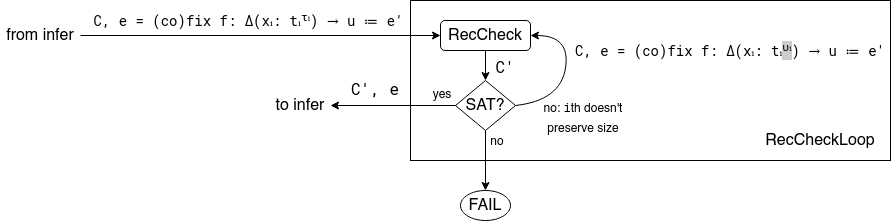
\includegraphics[width=\textwidth]{images/RecCheckLoop.png}
\caption{Illustration of simplification of \RecCheckLoop}
\label{fig:RecCheckLoop}
\end{figure}
\begin{figure}
\centering

\begin{minted}[escapeinside=<>,mathescape=true]{ocaml}
let rec RecCheckLoop <$C$> <$\Gamma$> <$\overline{\tau_k}$> <$\overline{t_k}$> <$\overline{e_k}$> =
  try let <$C'$> = <$\set{}$> in
    let for i = 1 to k do
      let pv<$_i$> = <$\PV$> <${t_i}$> in (* noninfinite $V^{\ast}$ *)
      let sv<$_i$> = (<$\SV$> <$\Gamma$> <$\cup$> <$\SV$> <$t_i$> <$\cup$> <$\SV$> <$e_i$>) <$\setminus$> pv<$_i$> in (* infinite $V^{\neq}$ *)
      <$C'$> := <$C'$> <$\cup$> RecCheck <$C$> <$\tau_i$> pv<$_i$> sv<$_i$>
    done in <$C'$>
  with RecCheckFail <$V$> ->
    if (empty? <$V$>)
    then raise RecCheckLoopFail
    else <$\mathcal{V}^*$> := <$\mathcal{V}^* \setminus V$>; RecCheckLoop <$C$> <$\overline{\tau_k}$> <$\overline{t_k}$> <$\overline{e_k}$>
\end{minted}

\caption{Pseudocode implementation of \RecCheckLoop}
\label{fig:helpers}
\end{figure}

%%% Local Variables:
%%% TeX-master: "../main.tex"
%%% TeX-engine: default
%%% End:


Lastly, we need to check that the constraint set so far is satisfiable.
However, \setrecstars and \setcorecstars optimistically annotate \textit{all} possible \coinductive types in the \cofixpoint type with position annotations, while not all \cofixpoints are size-preserving.
Therefore, instead of calling \RecCheck directly to check satisfiability,
\RecCheckLoop iteratively calls \RecCheck and discards incorrect position annotations at each iteration.
A simplification of the algorithm, not handling mutual \cofixpoints and removing single position annotations at a time,
is illustrated in \autoref{fig:RecCheckLoop}.
The size variable $\upsilon_i$ highlighted in grey corresponds to turning the position size variable into a regular size variable.

More precisely, \RecCheck either returns a new constraint set,
or it fails with some set $V$ of position size variables that must be set to infinity
and therefore mark arguments that are not size-preserving.
If $V$ is empty, then \RecCheckLoop fails overall: this indicates that the overall constraint set is unsatisfiable.
If $V$ is not empty, then we can try \RecCheck again after removing the size variables in $V$ from our set of position size variables,
thus no longer enforcing that they must be size-preserving.
An OCaml-like pseudocode implementation of \RecCheckLoop is provided by \autoref{fig:helpers}.

\subsection{RecCheck}\label{sec:algorithm:reccheck}

As in previous work on \CChatomega with coinductive streams~\citep{cc-hat-omega} and in \CIChat, we use the same \RecCheck algorithm from \Fhat~\citep{f-hat}.
This algorithm attempts to ensure that the subsizing rules in \autoref{fig:subsizing} can be satisfied within a given set of constraints.
It does so by checking the set of constraints for invalid circular subsizing relations, setting the size variables involved in the cycles to $\infty$, and producing a new set of constraints without these problems; or it fails, indicating nontermination or nonproductivity.
It takes four arguments:

\begin{itemize}
  \item A constraint set $C$, which we treat as a constraint graph.
  \item The size variable $\tau$ of the annotation on the type of the recursive argument (for fixpoints) or on the return type (for cofixpoints). While the return type (for fixpoints) or the types of other arguments (for cofixpoints) may optionally be marked as size-preserving, each \cofixpoint type requires at \textit{least} $\tau$ for the primary \corecursive type.
  \item A set of size variables $V^*$ that must be set to some non-infinite size.
    These are the size annotations in the \cofixpoint type that have position size variables.
    Note that $\tau \in V^*$.
  \item A set of size variables $V^\neq$ that must be set to $\infty$.
    These are all other non-position size annotations, found in the \cofixpoint types and bodies.
\end{itemize}

The key idea of the algorithm is that if there is a negative cycle in $C$,
then for any size variable $\upsilon$ in the cycle,
supposing that the total weight going once around the cycle is $-n$,
by transitivity we have the subsizing relation $\succ{\upsilon}^{n} \sqsubseteq \upsilon$,
This relation can only hold if $\upsilon = \infty$,
since $\succ{\infty} \sqsubseteq \infty$.
The algorithm proceeds as follows:

\begin{enumerate}
  \item \label{item:reccheck:smallest} Let $V^\iota = \bigsqcap V^*$, and add $\tau \sqsubseteq V^\iota$ to $C$.
    This ensures that $\tau$ is the smallest size variable among all the noninfinite size variables.
  \item \label{item:reccheck:neg-cycles} Find all negative cycles in $C$, and let $V^-$ be the set of all size variables in some negative cycle.
  \item Remove all edges with size variables in $V^-$ from $C$, and add $\infty \sqsubseteq V^-$.
  \item \label{item:reccheck:infty} Add $\infty \sqsubseteq \left(\bigsqcup V^\neq \cap \bigsqcup V^\iota\right)$ to $C$.
  \item \label{item:reccheck:bot} Let $V^\bot = \left(\bigsqcup \set{\infty}\right) \cap V^\iota$.
    This is the set of size variables that we have determined to both be infinite and noninfinite.
    If $V^\bot$ is empty, then return $C$.
  \item \label{item:reccheck:fail} Otherwise, let $V = V^\bot \cap (V^* \setminus \set{\tau})$, and fail with $\RecCheckFail{V}$.
    This is the set of contradictory position size variables excluding $\tau$, which we can remove from $\V^*$ in \RecCheckLoop.
    If $V$ is empty, there are no position size variables left to remove, so the check and therefore the size inference algorithm fails.
\end{enumerate}

Disregarding closure operations and set operations like intersection and difference, the time complexity of a single pass is $O(\norm{V}\norm{C})$, where $V$ is the set of size variables appearing in $C$.
This comes from the negative-cycle finding in (\ref{item:reccheck:neg-cycles}) using, for instance, the Bellman--Ford algorithm.

\begin{figure}
\centering

\begin{flushleft}
\fbox{$\Gamma_G^\circ \rightsquigarrow \Gamma_G$}
\end{flushleft}

\vspace{-3ex}

\begin{mathpar}
\inferrule*[right=\defrule{a-global-nil}]{~}{
    \square \rightsquigarrow \square
}
\and
\inferrule*[right=\defrule{a-global-assum}]{
    \Gamma_G^\circ \rightsquigarrow \Gamma_G \\
    \emptyset, \Gamma_G, \square \vdash t^\circ \rightsquigarrow \_, t \Rightarrow^* \varw
}{
    \Gamma_G^\circ(\Assm{x}{t^\circ\!\!}) \rightsquigarrow \Gamma_G(\Assm{x}{|t|^\infty\!\!})
}
\and
\inferrule*[right=\defrule{a-global-def}]{
    \Gamma_G^\circ \rightsquigarrow \Gamma_G \\
    \emptyset, \Gamma_G, \square \vdash t^\circ \rightsquigarrow C_1, t \Rightarrow^* \varw \\\\
    C_1, \Gamma_G, \square \vdash e^\circ \Leftarrow t \rightsquigarrow C_2, e \\
    \rho = \solve{C_2}
}{
    \Gamma_G^\circ(\Defn{x}{t^\circ}{e^\circ\!\!}) \rightsquigarrow \Gamma_G(\Defn{x}{\rho t}{\rho e})
}
\end{mathpar}
    
\caption{Size inference algorithm: Well-formedness}
\label{fig:algorithm-wf}
\end{figure}


\subsection{Well-Formedness}\label{sec:algorithm:wf}

A self-contained chunk of code, be it a file or a module, consists of a sequence of \coinductive definitions (signatures) and programs (global declarations).
For our purposes, we assume that there is a singular well-formed signature defined independently.
Then we need to perform size inference on each declaration of $\Gamma_G$ in order.
This is given by Rules \refnorule{a-global-nil}, \refnorule{a-global-assum}, and \refnorule{a-global-def} in \autoref{fig:algorithm-wf}.

In \refrule{a-global-def}, the \solve metafunction takes the constraint set $C_1 \cup C_2$
and produces a size substitution that, when applied to the annotated term and type, 
ensures that they form a well-typed judgement.
In other words, we are guaranteed that $\Sigma, \Gamma_G, \mt \vdash \rho e : \rho t$ holds.

Assuming for now that the corresponding constraint graph has no negative cycles, for every connected component,
the simplest solution is to assign size expressions to each size variable such that
all of those size expressions have the same base size variable.
For instance, given the constraint set $\set{\upsilon_1 \sqsubseteq \hat{\upsilon}_2, \hat{\upsilon_1} \sqsubseteq \upsilon_3}$,
one solution could be the mapping $\set{\upsilon_1 \mapsto \tau, \upsilon_2 \mapsto \tau, \upsilon_3 \mapsto \hat{\tau}}$.

This kind of problem is a \emph{difference constraint} problem \citep{clrs}.
Generally a solution involves finding a mapping from variables to integers, whereas our solution will map from size variables to size expressions with the same base, but the technique using a single-source shortest-path algorithm still applies.
Given a connected component $C_c$ with no negative cycles or an $\infty$ vertex, our algorithm $\solvecomp$ for finding a solution proceeds as follows:

\begin{enumerate}
  \item Generate a fresh size variable $\tau$.
  \item For every size variable $\upsilon_i$ in $C_c$, add an edge $\tau \sqsubseteq \upsilon_i$ of weight $0$.
  \item \label{item:solvecomp:shortest-path} Find the weights $w_i$ of the shortest paths from $\tau$ to every other size variable $\upsilon_i$ in $C_c$.
    This yields the constraint $\tau \sqsubseteq \hat{\upsilon}_i^{w_i}$.
  \item Na\"ively, we would map each $\upsilon_i$ to the size expression $\hat{\tau}^{-w_i}$
    to trivially satisfy $\tau \sqsubseteq \hat{\upsilon}_i^{w_i}$,
    since this would become $\tau \sqsubseteq \tau$ after substitution.
    However, $-w_i$ may be negative, which would make no sense as the size of a size variable.
    Therefore, we find the largest weight $w_{\max} \coloneqq \max_i w_i$, and shift all the sizes up by $w_{\max}$.
    In other words, we return the map $\rho \coloneqq \set{\upsilon_i \mapsto \hat{\tau}^{w_{\max} - w_i}}$.
\end{enumerate}

Again, the time complexity of a single pass is $O(\norm{V}\norm{C_c})$ (where $V$ is the set of size variables in $C_c$)
due to
finding the single-source shortest paths in (\ref{item:solvecomp:shortest-path}) using,
for instance, the Bellman--Ford algorithm.
(Note that although there are no negative cycles, there are still negative \emph{weights}, so we cannot use, for example, Dijkstra's algorithm.)
The total $\solve$ algorithm, given some constraint graph $C$, is then as follows:

% Is removing negative cycles necessary? Could we prove that there are *no* negative cycles?
\begin{enumerate}
  \item Initialize an empty size substitution $\rho$.
  \item Find all negative cycles in $C$, and let $V^-$ be all size variables in some negative cycle.
  \item Let $V^\infty = \bigsqcup \set{\infty}$.
  \item Remove all edges with size variables in $V^- \cup V^\infty$ from $C$, and for every $\upsilon_i \in V^- \cup V^\infty$, add $\upsilon_i \mapsto \infty$ to $\rho$.
  \item For every connected component $C_c$ of $C$, add mappings $\solvecomp{C_c}$ to $\rho$.
\end{enumerate}

Since dividing the constraint graph into connected components partitions the size variables and constraints into disjoint sets,
the time complexity of all executions of \solvecomp is $O(\norm{V}\norm{C})$.
This is also the time complexity of negative-cycle finding.
These two dominate the time complexity of finding the connected components,
which is $O(\norm{V} + \norm{C})$.

The resulting size substitution $\rho$ will then satisfy $\rho \vDash C$.
As we will see in the following subsection,
with soundness this implies that $\Sigma, \Gamma_G, \mt \vdash \rho e : \rho t$ holds.

\todo: What was the point?

\subsection{Metatheory}\label{sec:algorithm:metatheory}

In this subsection, we focus on soundness and completeness theorems of various parts of the inference algorithm.
The proof sketches and partial proofs for these and for the intermediate lemmas and theorems can be found in \autoref{sec:proofs}.

We first need soundness and completeness of \RecCheck.
The constraint set returned by \RecCheck ensures that variables that should be infinite are constrained to be so,
and that variables that shouldn't be infinite are not.
Intuitively, soundness then says that if you have a solution to a constraint set returned by \RecCheck,
then there must also be a solution to the original constraint set
that also ensures the same things.
Dually, completeness says that if you have a solution to the original constraint set that ensures these constraints,
then it must also be a solution to the constraint set returned by \RecCheck.

\begin{theorem}[Soundness of \RecCheck (SRC)]
If $\RecCheck(C', \tau, V^*, V^\neq) = C$, for every $\rho$ such that $\rho \vDash C$,
given a fresh size variable $\upsilon$, there exists a $\rho'$ such that the following all hold:
\begin{enumerate}
  \item $\rho' \vDash C'$;
  \item $\rho'\tau = \upsilon$;
  \item $\floor{\rho' V^*} = \upsilon$;
  \item $\floor{\rho' V^\neq} \neq \upsilon$;
  \item For all $\upsilon' \in V^\neq$, $(\set{\upsilon \mapsto \rho\tau} \circ \rho')(\upsilon') = \rho\upsilon'$; and
  \item For all $\tau' \in V^*$, $(\set{\upsilon \mapsto \rho\tau} \circ \rho')(\tau') \sqsubseteq \rho\tau'$.
\end{enumerate}
\end{theorem}

\begin{theorem}[Completeness of \RecCheck (CRC)]~\\
Suppose the following all hold:
\begin{itemize}
  \item $\rho \vDash C'$;
  \item $\rho\tau = \upsilon$;
  \item $\floor{\rho V^*} = \upsilon$; and
  \item $\floor{\rho V^\neq} \neq \upsilon$.
\end{itemize}
Then $\rho \vDash \RecCheck(C', \tau, V^*, V^\neq)$.
\end{theorem}

\RecCheck returns a constraint set for a single \cofixpoint definition with a fixed set of position variables;
\RecCheckLoop, on the other hand, returns a constraint set for an entire mutual \cofixpoint definition, finding a suitable set of position variables.
There are then two properties we want to ensure.

\begin{theorem}[Correctness of RecCheckLoop]~\\[-4ex]
\begin{enumerate}
  \item \RecCheckLoop terminates on all inputs.
  \item If $\RecCheckLoop{C', \Gamma, \vec{\tau_k}, \vec{t_k}, \vec{e_k}} = C$ with an initial position variable set $\mathcal{V}^*$,
  then for every $i \in \vec{k}$, $\RecCheck{C', \tau_i, \PV(t_i), \SV(\Gamma, t_i, e_i) \setminus \PV(t_i)} \subseteq C$ with a final position variable set $\mathcal{V}^*_\subseteq \subseteq \mathcal{V}^*$.
\end{enumerate}
\end{theorem}

We also want to ensure that \solvecomp and \solve actually return solutions of the constraint sets they are solving.

\begin{theorem}[Correctness of \solve and \solvecomp]~\\[-4ex]
\begin{enumerate}
  \item If the constraint set $C_c$ contains no negative cycles, then $\solvecomp{C_c} \vDash C_c$ and
  \item $\solve{C} \vDash C$.
\end{enumerate}
\end{theorem}

Before proceeding onto the main soundness theorems, we need a few lemmas ensuring that the positivity/negativity judgements
and algorithmic subtyping are sound and complete with respect to subtyping.

\begin{lemma}[Soundness of positivity/negativity]
Suppose that $\forall \upsilon \in \SV{t}, \rho_1 \upsilon \sqsubseteq \rho_2 \upsilon$.
\begin{enumerate}
  \item If $\gg \vdash \upsilon \pos t$, then $\gg \vdash \rho_1 t \leq \rho_2 t$; and
  \item If $\gg \vdash \upsilon \neg t$, then $\gg \vdash \rho_2 t \leq \rho_1 t$.
\end{enumerate}
\end{lemma}

\begin{lemma}[Completeness of positivity/negativity]~\\[-4ex]
\begin{enumerate}
  \item If $\Gamma_G, \Gamma \vdash t \leq \subst{t}{\upsilon}{\succ{\upsilon}}$ then $\gg \vdash \upsilon \pos t$.
  \item If $\Gamma_G, \Gamma \vdash \subst{t}{\upsilon}{\succ{\upsilon}} \leq t$ then $\gg \vdash \upsilon \neg t$.
\end{enumerate}
\end{lemma}

\begin{lemma}[Soundness of algorithmic subtyping]
Let $\Gamma_G, \Gamma \vdash t \constrain u \rightsquigarrow C$,
and suppose that $\rho \vDash C$.
Then $\Gamma_G, \rho \Gamma \vdash \rho t \leq \rho u$.
\end{lemma}

Now we are ready to tackle the main theorems, in particular soundness of checking, inference, and well-formedness
with respect to the typing rules.
We leave completeness of checking and inference as a conjecture,
but show that if it holds, then completeness of well-formedness will hold as well.

\begin{theorem}[Soundness (check/infer)]
Let $\Sigma$ be a fixed, well-formed signature, $\Gamma_G$ a global environment, $\Gamma$ a local environment, and $C$ a constraint set.
Suppose we have the following:
\begin{enumerate}[label=\alph*)]
  \item $\forall \rho \vDash C, \WF{\Gamma_G, \rho \Gamma}$.
  \item If $\Gamma \equiv \Gamma_1 (\defn{x}{t}{e}) \Gamma_2$ then $\forall \upsilon \in \SV(e, t), \upsilon \notin \SV(\Gamma_G, \Gamma_1)$.
\end{enumerate}
Then the following hold:
\begin{enumerate}
  \item If $C, \gg \vdash e^\circ \Leftarrow t \rightsquigarrow C', e$,
  then $\forall \rho' \vDash C \cup C'$,
  we have $\Gamma_G, \rho\Gamma \vdash \rho e : \rho t$.
  \item If $C, \gg \vdash e^\circ \rightsquigarrow C', e \Rightarrow t$,
  then $\forall \rho \vDash C \cup C'$,
  we have $\Gamma_G, \rho\Gamma \vdash \rho e : \rho t$.
\end{enumerate}
\end{theorem}

\begin{conjecture}[Completeness (check/infer)]
Let $\Sigma$ be a fixed, well-formed signature, $\Gamma_G$ a global environment, $\Gamma$ a local environment, $C$ a constraint set, and $\rho \vDash C$ a solution to the constraint set.
\begin{enumerate}
  \item If $\Gamma_G, \rho\Gamma \vdash e : \rho t$,
    then there exist $C', \rho'$ such that:
    \begin{itemize}
      \item $\rho' \vDash C'$;
      \item $\forall \upsilon \in \SV(\Gamma, t), \rho \upsilon = \rho' \upsilon$; and
      \item $C, \Gamma_G, \Gamma \vdash \erase{e} \Leftarrow t \rightsquigarrow C', e'$ where $\Gamma_G, \Gamma \vdash \rho' e' \conv* e$.
    \end{itemize}
  \item If $\Gamma_G, \rho\Gamma \vdash e : t$,
    then there exist $C, \rho'$ such that:
    \begin{itemize}
      \item $\rho' \vDash C'$;
      \item $\forall \upsilon \in \SV(\Gamma, t), \rho \upsilon = \rho' \upsilon$; and
      \item $C, \Gamma_G, \Gamma \vdash \erase{e} \rightsquigarrow C', e' \Rightarrow t'$ where $\Gamma_G, \Gamma \vdash \rho' e' \conv* e$ and $\Gamma_G, \Gamma \vdash \rho' t \leq t$.
    \end{itemize}
\end{enumerate}
\end{conjecture}

\begin{theorem}[Soundness (well-formedness)]
If $\Gamma_G^\circ \rightsquigarrow \Gamma_G$ then $\WF{\Gamma_G, \mt}$.
\end{theorem}

The completeness theorem for well-formedness is slightly different than expected:
a well-formed global environment, when erased, should successfully have sizes inferred,
but we don't place any requirements on the newly size-inferred environment,
just that there should be \emph{some} answer.

\begin{theorem}[Completeness (well-formedness)]
If $\WF{\Gamma_G, \mt}$ then $\erase{\Gamma_G} \rightsquigarrow \Gamma'_G$.
\end{theorem}

%%% Local Variables:
%%% TeX-master: "../main.tex"
%%% TeX-engine: default
%%% End:
